\documentclass[utf8,utf8x]{beamer}

\usepackage{listings}

\title{Scala development up and running with giter8}
\author{José Miguel Martínez Carrasco}
\institute[Springer]{Springer}
\date{\today}

\setbeamercolor{postit}{fg=black,bg=white!80!black}
\usetheme{Pittsburgh}
\usecolortheme{fly}

\logo{
\includegraphics[height=0.5cm]{springer_horse.png}}

% scala: http://tihlde.org/~eivindw/latex-listings-for-scala/
% "define" Scala
\lstdefinelanguage{scala}{
  morekeywords={abstract,case,catch,class,def,%
    do,else,extends,false,final,finally,%
    for,if,implicit,import,match,mixin,%
    new,null,object,override,package,%
    private,protected,requires,return,sealed,%
    super,this,throw,trait,true,try,%
    type,val,var,while,with,yield},
  otherkeywords={=>,<-,<\%,<:,>:,\#,@, <+=},
  sensitive=true,
  morecomment=[l]{//},
  morecomment=[n]{/*}{*/},
  morestring=[b]",
  morestring=[b]',
  morestring=[b]"""
}

\usepackage{color}
\definecolor{dkgreen}{rgb}{0,0.6,0}
\definecolor{gray}{rgb}{0.5,0.5,0.5}
\definecolor{mauve}{rgb}{0.58,0,0.82}
 
% Default settings for code listings
\lstset{frame=tb,
  language=scala,
  aboveskip=3mm,
  belowskip=3mm,
  showstringspaces=false,
  columns=flexible,
  basicstyle={\small\ttfamily},
  numbers=left,
  numberstyle=\tiny\color{gray},
  keywordstyle=\color{blue},
  commentstyle=\color{dkgreen},
  stringstyle=\color{mauve},
  frame=single,
  breaklines=true,
  breakatwhitespace=true
  tabsize=3
}

\begin{document}
\frame{\maketitle}

\section{Introduction}
\frame{\tableofcontents[currentsection]}

\subsection{Motivation}
\frame{
  \begin{description}
    \item[context] New technology, new tools, too many options.
    \item[target] Simple and working solution. 
  \end{description}
}

\section{Setup}
\frame{\tableofcontents[currentsection]}

\frame{
  \begin{beamercolorbox}[shadow=true, rounded=true]{postit}
  Everything under \$HOME/bin!!!
  \end{beamercolorbox}

  \begin{center}
  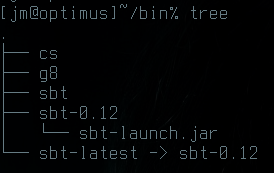
\includegraphics[scale=0.6]{binfolder.png}
  \end{center}
}

\subsection{requisites}
\frame{
  \begin{itemize}
    \item git
    \item github account
    \item unix
  \end{itemize}
}

\subsection{sbt}
\begin{frame}[fragile]
  \begin{lstlisting}[language=bash]
    #!/bin/sh    
    java -Xmx1024M -jar `dirname $0`/sbt-latest/sbt-launch.jar "$@" 
  \end{lstlisting} \cite{sbt}
\end{frame}

\subsection{giter8}
\frame{
  \begin{beamercolorbox}[shadow=true, rounded=true]{postit}
  	\textit{Giter8} is a command line tool to generate files and directories from templates published on github. It's implemented in Scala and runs through the Simple Build Tool launcher, but it can produce output for any purpose. \cite{g8}
  \end{beamercolorbox}
}

\subsection{conscript}
\begin{frame}[fragile]
  \begin{beamercolorbox}[shadow=true, rounded=true]{postit}
    \textit{Conscript} is a tool for installing and updating Scala software programs. \cite{cs}
  \end{beamercolorbox}

  \begin{lstlisting}[language=bash]
    curl https://raw.github.com/n8han/conscript/master/ \\
      setup.sh | sh
  
    cs n8han/giter8  
  \end{lstlisting}
\end{frame}

\section{Usage}
\frame{\tableofcontents[currentsection]}

\subsection{templates}
\begin{frame}[fragile]
  \begin{beamercolorbox}[shadow=true, rounded=true]{postit}
  Any github repository with g8 suffix.
  \end{beamercolorbox}

  \begin{lstlisting}[language=bash]
    g8 softprops/unfiltered
  \end{lstlisting}
\end{frame}

\subsection{publish}
\frame{
  \begin{beamercolorbox}[shadow=true, rounded=true]{postit}
  Publish your template as \textit{yourtemplate.g8} to github and update giter8 wiki \cite{g8templates}.
  \end{beamercolorbox}
}  

\section{References}
\frame{\tableofcontents[currentsection]}

\frame{
\begin{thebibliography}{10}
  \bibitem{sbt}{http://www.scala-sbt.org}
  \bibitem{g8}{https://github.com/n8han/giter8}
  \bibitem{cs}{https://github.com/n8han/conscript}
  \bibitem{g8templates}{https://github.com/n8han/giter8/wiki/giter8-templates}
\end{thebibliography}
}

\section*{Outline}
\frame{\tableofcontents}

\end{document}
